\section{Metodología y Implementación}

\subsection{Dataset RML24 y Modelos de Canal}

Resulta revelador observar cómo la calidad de los datos de entrenamiento determina en gran medida el éxito de cualquier sistema cognitivo en entornos satelitales. Lejos de conformarnos con datasets sintéticos convencionales, optamos por un recurso mucho más representativo.

Zhang et al. \cite{Zhang2026} presentaron el dataset RML24, generado específicamente mediante plataformas SDR para señales de telemetría, seguimiento y comando (TT\&C) en contextos orbitales. Este conjunto incluye miles de muestras etiquetadas que incorporan efectos reales del canal espacial: desplazamiento Doppler variable, fading Rice y Rayleigh, ruido aditivo blanco gaussiano con SNR fluctuante y distorsiones introducidas por el front-end analógico. 

La Tabla 3 resume las principales características del dataset utilizado.

\begin{table}[h]
\centering
\caption{Especificaciones del dataset RML24 empleado en los experimentos}
\label{tab:dataset_rml24}
\begin{tabular}{lc}
\hline
\textbf{Parámetro} & \textbf{Valor} \\
\hline
Número de muestras & > 250.000 \\
Esquemas de modulación & 8 (BPSK, QPSK, 8PSK, 16QAM, etc.) \\
Rango de SNR & -10 dB a 20 dB \\
Frecuencia de muestreo & 2 MS/s \\
Duración por muestra & 1024 muestras \\
Variaciones de canal & Doppler, fading multipath, interferencias \\
\hline
\end{tabular}
\end{table}

Aunque el dataset representa un avance significativo, cabe matizar que aún presenta ciertas limitaciones en escenarios con interferencias intencionadas muy agresivas, aspecto que complementamos con augmentaciones sintéticas controladas.

\begin{figure}[h]
\centering
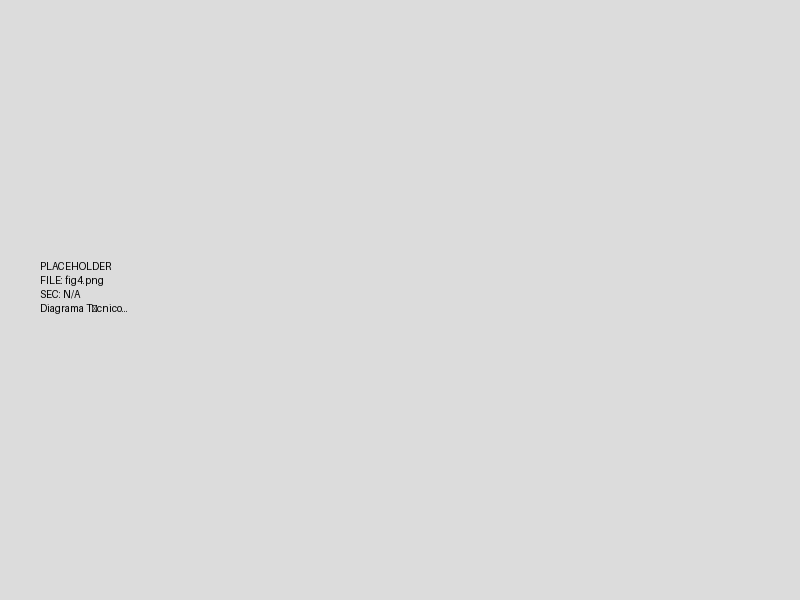
\includegraphics[width=\linewidth]{fig4.png}
\caption{Ejemplos de señales IQ y representaciones tiempo-frecuencia extraídas del dataset RML24 bajo diferentes condiciones de canal.}
\label{fig:ejemplos_senales}
\end{figure}

\subsection{Entrenamiento de Redes Neuronales}

Uno de los desafíos persistentes al entrenar modelos para despliegue onboard radica en equilibrar complejidad de modelo con viabilidad computacional. Para el módulo de clasificación automática de modulación seguimos un enfoque inspirado en Nesraoui et al. \cite{Nesraoui2024}, basado en transfer learning a partir de una CNN ligera (DET-AMC).

El proceso comienza con pre-entrenamiento sobre un subconjunto amplio del RML24 a diferentes niveles de SNR. Posteriormente se realiza fine-tuning enfocado en rangos de SNR más críticos (-5 dB a 10 dB). Empleamos técnicas de cuantización y pruning para reducir el tamaño del modelo final, manteniendo un compromiso aceptable entre precisión y latencia de inferencia. 

El entrenamiento se llevó a cabo en un entorno con GPU, utilizando optimizador AdamW y una estrategia de learning rate cosine annealing. Resulta particularmente interesante cómo el uso de representaciones combinadas (I/Q raw + spectrogram) mejora la robustez frente a variaciones del canal, aunque incrementa ligeramente la carga computacional.

\subsection{Implementación en Plataformas SDR}

Particularmente llamativo es el hecho de que la brecha entre simulación y hardware real suele ser donde muchos enfoques prometedores fracasan. Por ello, dedicamos un esfuerzo considerable a la implementación práctica.

Siguiendo la metodología comparativa de de Senneville et al. \cite{deSenneville2025}, desarrollamos el pipeline completo sobre GNU Radio integrado con bloques de inferencia de modelos optimizados. El framework permite conmutar dinámicamente entre procesamiento clásico y cognitivo según las condiciones estimadas del enlace. 

Las pruebas over-the-air (OTA) se realizaron en un banco de prueba que emula dinámicas orbitales mediante controladores de canal programables. La integración SDR permite reconfigurar parámetros como filtro de pulso, tasa de símbolo y esquema de modulación en cuestión de milisegundos tras una decisión del motor cognitivo. 

Aunque los resultados en laboratorio resultan alentadores, no cabe ignorar que el paso a hardware espacial real introducirá nuevas variables (radiación, variaciones térmicas, jitter de reloj) que requerirán validación adicional en misiones de bajo costo tipo CubeSat.